\chapter{Практическая часть}
\label{ch:chap2}

\section*{\textbf{Передача данных между Adalm Pluto и хостом}}

Передача данных (IQ-сэмплов) между Adalm Pluto и хост-компьютером осуществляется посредством USB 2.0. Важно отметить, 
что в случае с SDR, данные необходимо передавать непрерывно в обе стороны (с хост-компьютера на SDR и обратно) одновременно. 
Хоть и теоретическая пропускная способность USB 2.0 равна 480 Mb/s, работа в полудуплексном режиме с передачей данных в 
обе стороны одновременно (с точки зрения пользователя) разительно снижается. Целевое значение частоты дискретизации 
желательно задавать в пределах ~6 Msps.

\section*{\textbf{Timestamping}}

В библиотеке SoapySDR реализованы функции получения временных меток (timestamp) с FPGA (Xilinx Zynq). Временные метки (timestamp) привязаны к каждому запросу 
данных с буфера ПЛИС, что, в свою очередь, позволяет синхронно получать/передавать данные в потоках RX/TX. Более того, 
из-за проблем с пропускной способностю USB 2.0 возникает проблема увеличения частоты дескритизации, при больших значениях которой,
USB 2.0 не может обеспечить полноценную передачу и прием (одновременных) сэмплов из Adalm Pluto на хост-компьютер. 
Выявить данную проблему можно благодаря реализации функции временных меток с Xilinx Zynq.

\section*{\textbf{Установка необходимых библиотек и зависимостей}}

\textbf{SoapySDR}

SoapySDR — открытая обобщённая API и библиотека времени выполнения для взаимодействия с SDR-устройствами. 
С помощью SoapySDR можно создавать экземпляры, настраивать и вести потоковую передачу данных с SDR-устройством в различных средах.
Большинство готовых SDR-платформ поддерживаются SoapySDR, и многие открытые приложения используют SoapySDR для интеграции с 
оборудованием. Кроме того, SoapySDR имеет привязки к средам разработки, таким как GNU Radio и Pothos.

\begin{lstlisting}
sudo apt-get install python3-pip python3-setuptools
sudo apt-get install cmake g++ libpython3-dev python3-numpy swig python3-matplotlib

git clone --branch soapy-sdr-0.8.1 https://github.com/TelecomDep/SoapySDR.git

cd SoapySDR
mkdir build && cd build

cmake ../

make -j 16
sudo make install
sudo ldconfig
\end{lstlisting}

\textbf{Libiio}

libiio — библиотека, разработанная компанией Analog Devices, которая предназначена для упрощения работы с устройствами ввода-вывода
данных (I/O), особенно с программируемыми аналогово-цифровыми и цифро-аналоговыми преобразователями (ADC/DAC), а также с 
радиооборудованием на базе платформы ADI (например, ADALM-PLUTO). Позволяет читать и записывать данные в реальном времени.

\begin{lstlisting}
sudo apt-get install libxml2 libxml2-dev bison flex libcdk5-dev cmake
sudo apt-get install libusb-1.0-0-dev libaio-dev pkg-config 
sudo apt install libavahi-common-dev libavahi-client-dev


git clone --branch v0.24 https://github.com/TelecomDep/libiio.git

cd libiio
mkdir build && cd build
cmake ../
make -j 16
sudo make install
\end{lstlisting}

\textbf{LibAD9361}

LibAD9361 - библиотека для работы с радиочипами семейства AD9361 от Analog Devices. В сочетании с libiio позволяет организовать 
потоковое чтение/запись данных в реальном времени.

\begin{lstlisting}
git clone --branch v0.3 https://github.com/TelecomDep/libad9361-iio.git
cd libad9361-iio

mkdir build && cd build

cmake ../

make -j 16
sudo make install
sudo ldconfig
\end{lstlisting}

\textbf{SoapyPlutoSDR}

SoapyPlutoSDR - библиотека, которая является расширением библиотеки SoapySDR, предназначенная для работы конкретно с Adalm Pluto. 

\begin{lstlisting}
git clone --branch sdr_gadget_timestamping https://github.com/TelecomDep/SoapyPlutoSDR.git
cd SoapyPlutoSDR

mkdir build && cd build

cmake ../

make -j 16
sudo make install
sudo ldconfig
\end{lstlisting}

\section*{\textbf{Основне моменты работы с Adalm Pluto напрямую из C++}}

\subsection*{\textbf{Подключение библиотек}}

\begin{lstlisting}
// Init device
#include <SoapySDR/Device.h>  
// Data types for writing samples 
#include <SoapySDR/Formats.h>  
\end{lstlisting}

\subsection*{\textbf{Инициализация устройства}}

\begin{lstlisting}
//create struct for init
SoapySDRKwargs args = {};

//Select device type
SoapySDRKwargs_set(&args, "driver", "plutosdr");       
if (1) {
    // Sample transmission method (usb)
    SoapySDRKwargs_set(&args, "uri", "usb:");           
} else {
    // Or IP
    SoapySDRKwargs_set(&args, "uri", "ip:192.168.2.1"); 
}
SoapySDRKwargs_set(&args, "direct", "1");
// Buffer size and timestamps              
SoapySDRKwargs_set(&args, "timestamp_every", "1920");  
// Use antennas?
SoapySDRKwargs_set(&args, "loopback", "0");
// Init             
SoapySDRDevice *sdr = SoapySDRDevice_make(&args);    
// Free memory   
SoapySDRKwargs_clear(&args);
\end{lstlisting}

\subsection*{\textbf{Формирование потоков и буферов}}

\begin{lstlisting}
// create streams
SoapySDRStream *rxStream = SoapySDRDevice_setupStream(sdr, SOAPY_SDR_RX, SOAPY_SDR_CS16, channels, channel_count, NULL);
SoapySDRStream *txStream = SoapySDRDevice_setupStream(sdr, SOAPY_SDR_TX, SOAPY_SDR_CS16, channels, channel_count, NULL);

//start streaming
SoapySDRDevice_activateStream(sdr, rxStream, 0, 0, 0); 
SoapySDRDevice_activateStream(sdr, txStream, 0, 0, 0);


// Get RX/TX MTU sizes

size_t rx_mtu = SoapySDRDevice_getStreamMTU(sdr, rxStream);
size_t tx_mtu = SoapySDRDevice_getStreamMTU(sdr, txStream);

// allocate memory for buffers (for RX/TX samples)
int16_t tx_buff[2 *tx_mtu];
int16_t rx_buffer[2 *rx_mtu];
\end{lstlisting}


\subsection*{\textbf{Получение I/Q семплов}}

\begin{lstlisting}
// start receive samples
for (size_t buffers_read = 0; buffers_read < iteration_count; buffers_read++)
{
    void *rx_buffs[] = {rx_buffer};
    // flags set by receive operation
    int flags;    
    //timestamp for receive buffer   
    long long timeNs; 
    
    // Read samples from stream and write I/Q samples in file
    int sr = SoapySDRDevice_readStream(sdr, rxStream, rx_buffs, rx_mtu, &flags, &timeNs, timeoutUs);
    // write in file
    for(int i = 0; i < rx_mtu * 2; i++){
        fprintf(file, "%d %d\n", rx_buffer[i], rx_buffer[i+1]);
    }
}
\end{lstlisting}

\subsection*{\textbf{Освобождение памяти}}

\begin{lstlisting}
//stop streaming
SoapySDRDevice_deactivateStream(sdr, rxStream, 0, 0);
SoapySDRDevice_deactivateStream(sdr, txStream, 0, 0);

//shutdown the stream
SoapySDRDevice_closeStream(sdr, rxStream);
SoapySDRDevice_closeStream(sdr, txStream);

//cleanup device handle
SoapySDRDevice_unmake(sdr);
\end{lstlisting}

После работы программы создатся файл samples.txt, в котором будут храниться полученные семплы в формате: (I,Q). Для визуализации
I(t) и Q(t) напишем простой парсер на Python. Результат:

\begin{figure}[H]
    \centering
    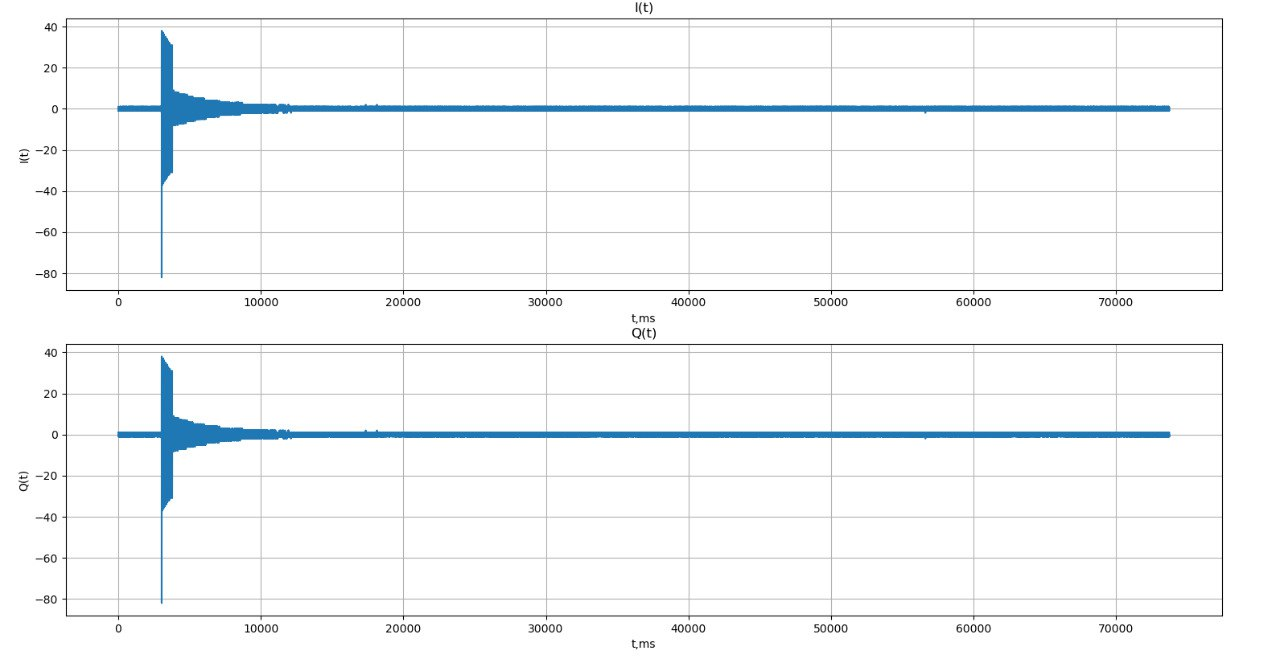
\includegraphics[width=0.8\textwidth]{ItQt.png}
    \caption{Графики I(t) и Q(t)}
\end{figure}

Можем наблюдать, что графики напонимают прямоугольный сигнал.

\endinput
